\section{High Level View}
Deep Learning is a Machine Learning area. A machine learns when after being exposed to data, it updates internal parameters making it more predictive. This process is depicted on the image. 

Machine Learning is - at least on this context -  a program that changes from exposure to data (experience).

\begin{figure}[h]
 \centering
 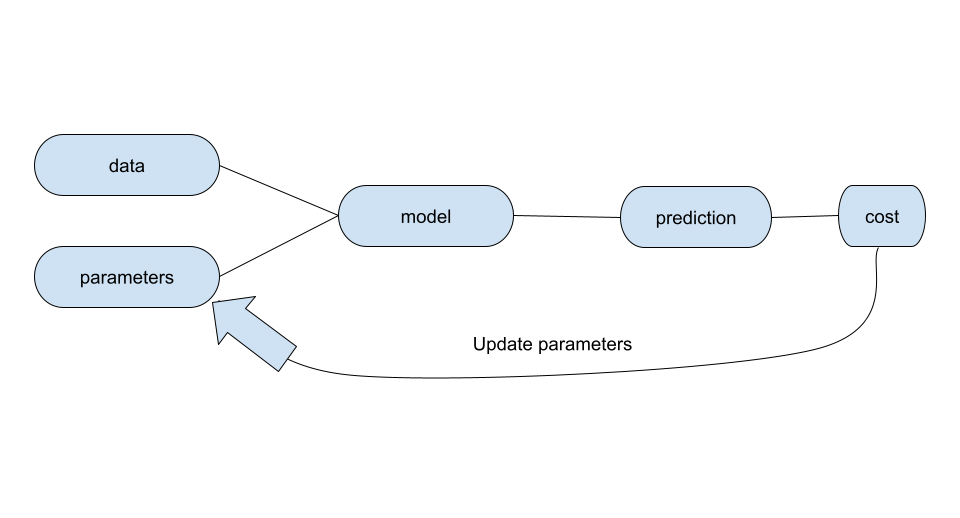
\includegraphics[width=0.9\textwidth]{ml.png}
 \caption{Machine Learning Process}
\end{figure}

Deep Learning models complex patterns of data. It's particularly useful for non-linear patterns. This opens up a new range of problems to solve. Because Deep Learning is a part of Machine Learning, the previous logic found in neural network diagrams (see Figures \ref{fig:single} and \ref{fig:shallow}).


\begin{figure}
 \centering
 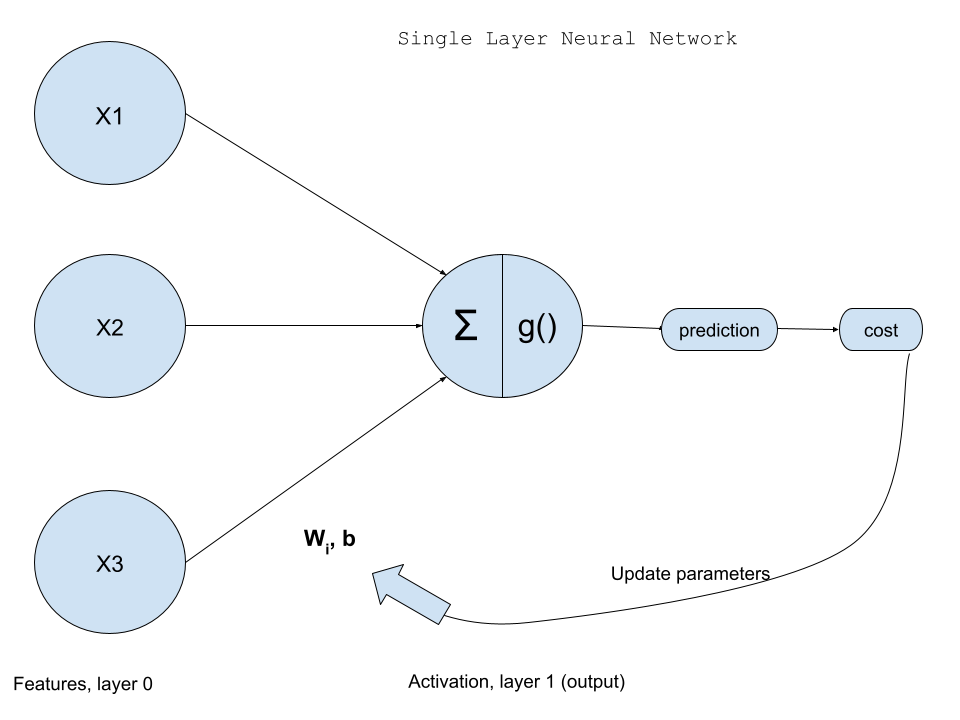
\includegraphics[width=\textwidth]{1L-NN.png}
 \caption{Single Layer Neural Network}
 \label{fig:single}
\end{figure}


\begin{figure}
 \centering
 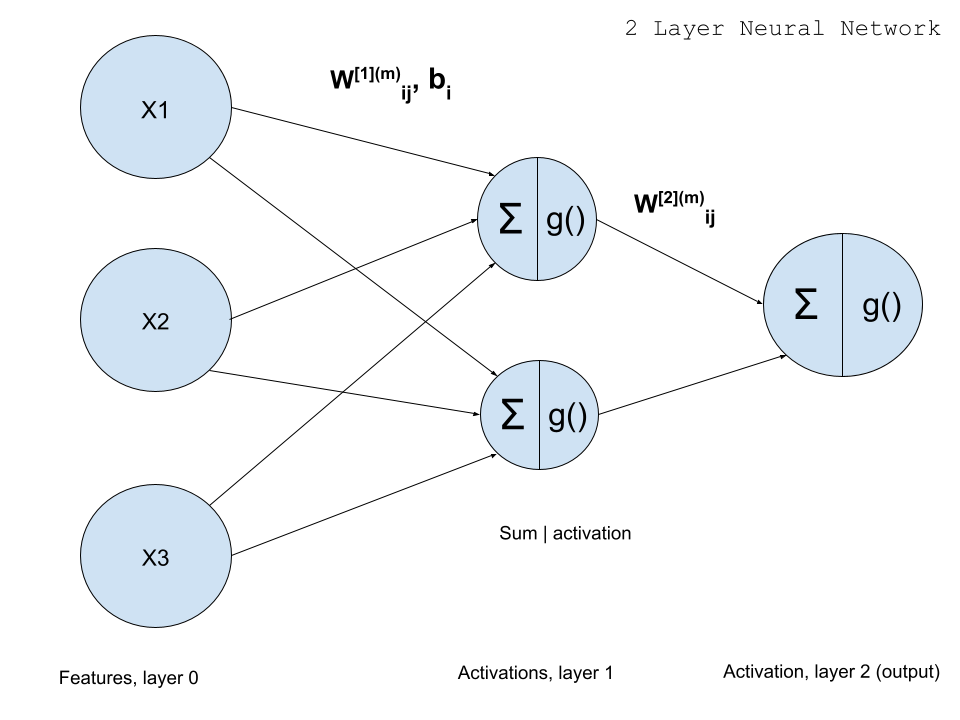
\includegraphics[width=\textwidth]{2L-NN.png}
 \caption{Shallow Neural Network}
 \label{fig:shallow}
\end{figure}

\section{The steps}
There are two main steps: \textit{forward} and \textit{backward} propagation. 

Suppose a mathematical function is given to us:
$$ y(x_1,x_2) = a x_1 + b x_2 + c$$
where $a$, $b$, $c$ are \textit{parameters}.

In \textit{Forward Propagation} we initialize a set of parameters (say $a,b,c=0$, and use an equation to estimate the output ($y$). We input the $y$ to another function ``$C$'' which is small if we're doing well, or large if bad.

In \textit{Backward Propagation} we minimize $C$, by differentiation, and find a way to move our function parameters towards the minimum. We use \textit{Gradient Descent}.

Basically, we run an estimation, compute $C$, and use this to update our function, iteratively.

We will see examples in detail, starting with multivariable linear regression, that is, a previous step to \textit{Deep Learning} and Neural Networks.
